\documentclass[10pt]{beamer}

\usetheme{metropolis}
\usepackage{appendixnumberbeamer}

\usepackage{booktabs}
\usepackage[scale=2]{ccicons}
\usepackage{graphicx}
\usepackage{hyperref}
\usepackage{circuitikz}
\usepackage{pdflscape}
\usepackage{smartdiagram}

\usepackage{color}
\usepackage{listings}

\lstset{
	basicstyle=\footnotesize\ttfamily,
    keepspaces=true,
    showstringspaces=false,
    language=PHP,
    commentstyle=\ttfamily,
}

\usepackage[OT4]{polski}
\usepackage[utf8]{inputenc}

\usepackage{pgfplots}
\usepgfplotslibrary{dateplot}

\usepackage{xspace}
\newcommand{\themename}{\textbf{\textsc{metropolis}}\xspace}

\setbeamertemplate{frame footer}{}
\setbeamertemplate{frame numbering}{}

\usetikzlibrary{shapes,arrows}

\tikzstyle{decision} = [diamond, draw, fill=blue!20, 
    text width=4.5em, text badly centered, node distance=3cm, inner sep=0pt]
\tikzstyle{block} = [rectangle, draw, fill=blue!20, 
    text width=5em, text centered, rounded corners, minimum height=4em]
\tikzstyle{line} = [draw, -latex']
\tikzstyle{cloud} = [draw, ellipse,fill=red!20, node distance=3cm,
    minimum height=2em]


\title{Wzorzec architektoniczny MVC}

\subtitle{Projektowanie i programowanie systemów internetowych I}
\author{mgr inż. Krzysztof Rewak}
\date{\today}
\institute{Wydział Nauk Technicznych i Ekonomicznych \\ Państwowa Wyższa Szkoła Zawodowa im. Witelona w Legnicy}

\begin{document}

\maketitle

\begin{frame}{Plan prezentacji}
  \setbeamertemplate{section in toc}[sections numbered]
  \tableofcontents[hideallsubsections]
\end{frame}


\section{Wzorce projektowe i architektoniczne}

\begin{frame}{Jak należy pisać kod?}
	„Jeżeli coś jest głupie, ale działa, to nie jest głupie.''
	
	\ \\
	
	Każdy student programowania wyznający taką zasadę powinien poważnie się zastanowić czy to faktycznie jest dziedzinia, w której chce się rozwijać.
\end{frame}

\begin{frame}{Jak należy pisać kod?}
	Tworzone oprogramowanie powinno być:
	\begin{itemize}
		\item czytelne,
		\item udokumentowane,
		\item zoptymalizowane względem redundancji i innych wybranych wskaźników,
		\item napisane zgodnie z konwencjami języka,
		\item napisane zgodnie z dobrymi praktykami programistycznymi,
		\item możliwe do rozwijania i rozszerzania.
	\end{itemize}
\end{frame}

\begin{frame}{Wynajdowanie koła na nowo}
	Prawda jest taka, że wiele problemów jakie często napotykają programiści, to problemy, które ktoś już kiedyś napotkał i najczęściej rozwiązał.
	
	Warto poznać sprawdzone rozwiązania, aby zaoszczędzić czasu przy budowaniu własnego systemu informatycznego. 
	
	Warto też jednak pamiętać, że wykorzystanie opracowanych wzorców to jedno, a budowanie aplikacji z gotowych wtyczek i bibliotek to coś całkiem innego!
\end{frame}

\begin{frame}{Wynajdowanie koła na nowo}
	Za Wikipedią:
	
	 Wzorce projektowe (\emph{design pattern}) to uniwersalne, sprawdzone w praktyce rozwiązania często pojawiających się, powtarzalnych problemów projektowych. Pokazują powiązania i zależności pomiędzy klasami oraz obiektami i ułatwiają tworzenie, modyfikację oraz pielęgnację kodu źródłowego.\textbf{ Są opisem rozwiązania, a nie jego implementacją.}
\end{frame}

\begin{frame}{Wzorce projektowe}
	Warto zainteresować się kilkoma popularnymi wzorcami:
	\begin{itemize}
		\item singleton,
		\item adapter,
		\item strategia,
		\item budowniczy,
		\item fabryka abstrakcyjna,
		\item wstrzykiwanie zależności.
	\end{itemize}
\end{frame}

\begin{frame}{A gdyby objąć wzorcem podwaliny całego systemu?}
	Gdy wzorce projektowe rozwiązują problemy zachodzące przede wszystkim między obiektami, wzorzec architektoniczny jest rozwiązaniem pomagającym na skalę całej aplikacji.
\end{frame}

\begin{frame}{Wzorce architektoniczne}
	Wzorce architektoniczne opisują:
	\begin{itemize}
		\item założenia architektury systemu,
		\item strukturę aplikacji,
		\item sposoby komunikacji wewnętrznej i zewnętrznej,
		\item funkcjonalności systemu.
	\end{itemize}
\end{frame}

\begin{frame}{Wzorce architektoniczne}
	Spośród popularnych wzorców można wymienić:
	\begin{itemize}
		\item ETL, \emph{extract-transform-load},
		\item P2P, \emph{peer-to-peer},
		\item ESB, \emph{enterprise service bus},
		\item EDA, \emph{event-driven architecture},
		\item szeroko rozumiane mikroserwisy...
	\end{itemize}
\end{frame}

\section{Idea MVC}

\begin{frame}{MVC?}
	Skrót \textbf{MVC} należy rozumień następująco:

	\textbf{M}odel - reprezentacja danych
	
	\textbf{V}iew, widok - warstwa prezentująca
	
	\textbf{C}ontroller, kontroler - obsługa zapytań
\end{frame}

\begin{frame}[fragile]{Podstawowy schemat interakcji}
	\hspace*{1.25cm}%
	\begin{tikzpicture}[node distance=4cm, minimum size=2cm, auto]
	
		\node [circle, fill=orange,inner sep=3pt] (user) {użytkownik};
		
		\node [block, above right of=user] (controller) {kontroler};
		\node [block, above left of=user] (view) {widok};
		\node [block, above left of=controller] (model) {model};
		
	
		\path [line] (user) -- node[label={[shift={(2,-3.5)}]wywołuje}] {} (controller);
		\path [line] (controller) -- node[label={[shift={(2,-0.5)}]żąda zmian}] {} (model);
		\path [line] (model) -- node[label={[shift={(-2,-0.5)}]uaktualnia}]  {} (view);
		\path [line] (view) -- node[label={[shift={(-2,-3.5)}]wyświetla}] {} (user);
	\end{tikzpicture}
\end{frame}

\begin{frame}{Występowanie}
	MVC to podstawowy wzorzec wykorzystywany w najpopularniejszych frameworkach:
	
	\begin{itemize}
		\item PHP: Laravel, Symfony, Phalcon, Yii
		\item ASP.NET MVC
		\item Java: Swing, Spring
		\item Ruby on Rails
		\item Django
	\end{itemize}
\end{frame}

\section{Reprezentacja danych}

\begin{frame}{Wielkie M}
	Model należy rozumieć jako reprezentację danych, pewną strukturę danych albo nawet sposób na pobieranie i zarządzanie danymi.
\end{frame}

\begin{frame}[fragile]{Wielkie M}
	\hspace*{1.25cm}%
	\begin{tikzpicture}[node distance=4cm, minimum size=2cm, auto]
	
		\node [circle, fill=orange,inner sep=3pt] (user) {użytkownik};
		
		\node [block, above right of=user] (controller) {kontroler};
		\node [block, above left of=user] (view) {widok};
		\node [block, fill=red, above left of=controller] (model) {model};
		
	
		\path [line] (user) -- node[label={[shift={(2,-3.5)}]wywołuje}] {} (controller);
		\path [line] (controller) -- node[label={[shift={(2,-0.5)}]żąda zmian}] {} (model);
		\path [line] (model) -- node[label={[shift={(-2,-0.5)}]uaktualnia}]  {} (view);
		\path [line] (view) -- node[label={[shift={(-2,-3.5)}]wyświetla}] {} (user);
	\end{tikzpicture}
\end{frame}

\begin{frame}[fragile]{Więc chodź, zamodeluj mój świat, na żółto i na niebiesko...}
	\begin{lstlisting}
<?php

use namespace App\Models;

class User {
  private $uid;
  private $login;
  private $password;
  
  public function __construct(string $login, string $password)
  {
    $this->id = uniqid();
    $this->login = $login;
    $this->password = password_hash($password, PASSWORD_BCRYPT);
  }
}
	\end{lstlisting}
\end{frame}

\begin{frame}[fragile]{Więc chodź, zamodeluj mój świat, na żółto i na niebiesko...}
	\begin{lstlisting}
from bcrypt import hashpw, gensalt
import uuid

class User(object):

  def __init__(self, name, password):
    self.id = uuid.uuid4()
    self.name = name
    self.password = hashpw(password, gensalt())
	\end{lstlisting}
\end{frame}

\begin{frame}{Skąd brać dane?}
	Dane do modelu można pobrać z różnych źródeł i wszystko tak naprawdę zależy od tego, czego potrzebuje aplikacja. Dane mogą pochodzić z:
	
	\begin{itemize}
		\item bazy danych,
		\item systemu pamięci podręcznej,
		\item z serializowanych obiektów,
		\item z plików,
		\item prosto z kodu.
	\end{itemize}
\end{frame}

\begin{frame}[fragile]{Co ten model robi?}
	Istnieją dwa podstawowe sposoby zarządzania modelami, ale o tym porozmawiamy przy okazji wykładu 9. \emph{Mapowanie relacyjno-obiektowe}.
	
	Klasyczny wzorzec MVC mówi, że model zawiera w sobie podstawową logikę biznesową. Dlatego na każdym obiekcie modelu powinno móc się wywoływać konkretne metody, np.:
	\begin{lstlisting}
public class Application
{
  public static void Main()
  {
    User user = new User("krewak", "secretpassword");
    user.SendNotificationEmail();
    user.ToggleStatus();
    user.Save();
  }
}
	\end{lstlisting}
\end{frame}

\begin{frame}{Zastrzeżenie!}
	Należy jednak pamiętać, że im większy system, tym bardziej skomplikowana staje się jego architektura. Często MVC rozszerza się o dodatkowe komponenty i wówczas pokazane przed chwilą podejście nie jest już prawidłowe.
\end{frame}

\section{Warstwa prezentująca}

\begin{frame}{Wielkie V}
	Widok należy rozumieć jako warstwę prezentującą, ale również umożliwiającą interakcję z systemem.
\end{frame}

\begin{frame}[fragile]{Wielkie V}
	\hspace*{1.25cm}%
	\begin{tikzpicture}[node distance=4cm, minimum size=2cm, auto]
	
		\node [circle, fill=orange,inner sep=3pt] (user) {użytkownik};
		
		\node [block, above right of=user] (controller) {kontroler};
		\node [block, fill=red, above left of=user] (view) {widok};
		\node [block, above left of=controller] (model) {model};
		
	
		\path [line] (user) -- node[label={[shift={(2,-3.5)}]wywołuje}] {} (controller);
		\path [line] (controller) -- node[label={[shift={(2,-0.5)}]żąda zmian}] {} (model);
		\path [line] (model) -- node[label={[shift={(-2,-0.5)}]uaktualnia}]  {} (view);
		\path [line] (view) -- node[label={[shift={(-2,-3.5)}]wyświetla}] {} (user);
	\end{tikzpicture}
\end{frame}

\begin{frame}[fragile]{Widok na widok}
	Poniżej widać dobry przykład odseparowania warstwy wizualnej za pomocą PHP-owego Twiga.
	
	\begin{lstlisting}
<table class="table">
  
    <tr data-user-id="{{ user.id }}">
      <td>{{ user.id }}</td>
      <td>{{ user.login }}</td>
      <td>{{ user.email }}</td>
      <td>{{ user.status }}</td>
      <td>
        <button class="btn btn-danger remove-user">
          delete
        </button>
      </td>
    </tr>  
  
</table>
	\end{lstlisting}
\end{frame}

\begin{frame}{Formy widoku}
	Widok najczęściej utożsamiany był w systemach internetowych z HTML-em, jednakże warstwą prezentacji może być cokolwiek, co zrozumie użytkownik lub inny system:	\begin{itemize}
		\item wspomniany HTML,
		\item XML,
		\item JSON,
		\item lub własny format lub standard.
	\end{itemize}
	
	Oczywiście HTML daje największe możliwości dla przeglądarki oraz możliwość łatwego wywołania kontrolera.
\end{frame}

\section{Obsługa zapytań}

\begin{frame}{Wielkie C}
	Kontroler należy przede wszystkim rozumieć jako obsługę zapytań. Jego podstawowym zadaniem jest przyjęcie zapytania od serwera HTTP oraz zwrócenie mu odpowiedzi.
\end{frame}

\begin{frame}[fragile]{Wielkie C}
	\hspace*{1.25cm}%
	\begin{tikzpicture}[node distance=4cm, minimum size=2cm, auto]
	
		\node [circle, fill=orange,inner sep=3pt] (user) {użytkownik};
		
		\node [block, fill=red, above right of=user] (controller) {kontroler};
		\node [block, above left of=user] (view) {widok};
		\node [block, above left of=controller] (model) {model};
		
	
		\path [line] (user) -- node[label={[shift={(2,-3.5)}]wywołuje}] {} (controller);
		\path [line] (controller) -- node[label={[shift={(2,-0.5)}]żąda zmian}] {} (model);
		\path [line] (model) -- node[label={[shift={(-2,-0.5)}]uaktualnia}]  {} (view);
		\path [line] (view) -- node[label={[shift={(-2,-3.5)}]wyświetla}] {} (user);
	\end{tikzpicture}
\end{frame}

\begin{frame}{Co może kontroler w MVC?}
	\begin{itemize}
		\item przyjąć dane wejściowe,
		\item znaleźć zbiór lub konkretny model oraz dokonać na nim zmian,
		\item przekierować na inny kontroler,
		\item zwrócić odpowiedź w formie widoku.
	\end{itemize}
\end{frame}

\begin{frame}[fragile]{Kontrolowanie kontrolerów}
	\begin{lstlisting}
<?php

namespace PWSZ\Controllers;

use Phalcon\Http\Response;

class NewsController extends Controller {

   public function getNewsAction(): Response {
      $this->dataset->setData(News::find())
      return $this->renderResponse();
   }

   public function getEntryAction(int $id): Response {
      $this->dataset->setData(News::findFirst($id))
      return $this->renderResponse();
   }

}
	\end{lstlisting}
\end{frame}

\begin{frame}{Co może kontroler poza MVC?}
	Wzorzec MVC jest bardzo popularną koncepcją, jednakże rzadko bywa używany w swojej klasycznej formie. Najczęstszymi rozszerzeniami są:
	\begin{itemize}
		\item serwisy, które wykonują logikę biznesową zamiast modeli,
		\item repozytoria, które zarządzają modelami,
		\item zdarzenia, które łamią jednokierunkowy przepływ zapytania,
		\item i inne - zależne od progrmiasty i wymagań systemu.
	\end{itemize}
\end{frame}

\begin{frame}[fragile]{Możliwe rozszerzenie systemu}
	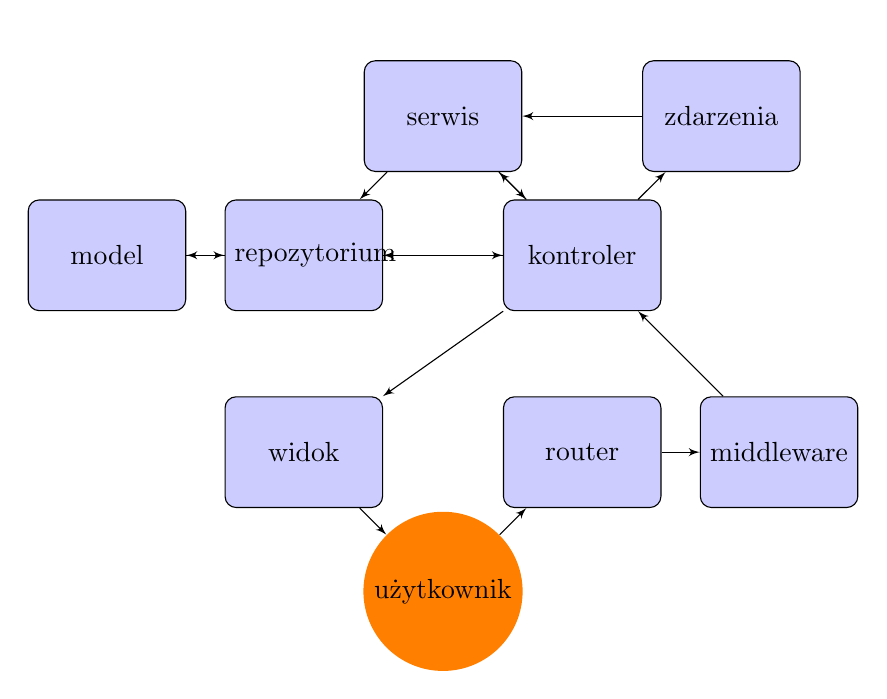
\begin{tikzpicture}[node distance=2.5cm, minimum size=2cm, auto]
	
		\node [circle, fill=orange,inner sep=3pt] (user) {użytkownik};
		
		\node [block, above right of=user] (router) {router};
		\node [block, above left of=user] (view) {widok};
		\node [block, right of=router] (middleware) {middleware};
		
		\node [block, above of=router] (controller) {kontroler};
		\node [block, above of=view] (repo) {repozytorium};
		\node [block, left of=repo] (model) {model};
		
		\node [block, above left of=controller] (service) {serwis};
		\node [block, above right of=controller] (event) {zdarzenia};
		
		\path [line] (user) -- node {} (router);
		\path [line] (router) -- node {} (middleware);
		\path [line] (middleware) -- node {} (controller);
		\path [line] (controller) -- node {} (service);
		\path [line] (controller) -- node {} (event);
		\path [line] (event) -- node {} (service);
		\path [line] (service) -- node {} (repo);
		\path [line] (controller) -- node {} (repo);
		\path [line] (repo) -- node {} (model);
		\path [line] (controller) -- node {} (view);
		\path [line] (view) -- node {} (user);
		
		\path [line] (service) -- node {} (controller);
		\path [line] (repo) -- node {} (controller);
		\path [line] (model) -- node {} (repo);
	\end{tikzpicture}
\end{frame}

\section{Podsumowanie}

\begin{frame}{Wady i zalety?}
	\begin{itemize}
		\item +/- popularność
		\item +/- separacja odpowiedzialności
		\item +/- złożoność systemu
		\item +/- testowanie
		\item +/- umożliwienie pracy \emph{full-stack developerom}
	\end{itemize}
\end{frame}

\begin{frame}{Bibliografia i ciekawe źródła}
  
	\begin{thebibliography}{9}
	
		\bibitem{wzorce}
		\url{https://pl.wikipedia.org/wiki/Wzorzec_projektowy_(informatyka)}
	
		\bibitem{wzorce-a}
		\url{https://pl.wikipedia.org/wiki/Wzorzec_architektoniczny}
	
		\bibitem{msdn}
		\url{https://msdn.microsoft.com/en-us/library/ff649643.aspx}
		
		\ \\ Wzorce w praktyce:
	
		\bibitem{php}
		\url{https://designpatternsphp.readthedocs.io/en/latest/}
	
		\bibitem{csharp}
		\url{http://www.inforsoft.nazwa.pl/inforsoft-nowy/kody-c/}
		
	\end{thebibliography}

\end{frame}

\appendix

\begin{frame}[standout]
	Pytania?
\end{frame}

\begin{frame}{}

	Kod prezentacji dostępny jest w repozytorium git pod adresem \texttt{https://bitbucket.org/krewak/pwsz-ppsi} \\ \ \\

	\begin{figure}
		\centering
		\href{https://bitbucket.org/krewak/pwsz-ppsi}{
			
\includegraphics[width=.15\textwidth]{../_template/bitbucket.png}
		}
	\end{figure}
	
	Wszystkie informacje dot. kursu dostępne są pod adresem \texttt{http://pwsz.rewak.pl/kursy/4} \\ \ \\

	\begin{figure}
		\centering
		\href{http://pwsz.rewak.pl/kursy/3}{
			
\includegraphics[width=.15\textwidth]{../_template/rewak.png}
		}
	\end{figure}

\end{frame}

\end{document}
